\section{Experimental results}
\label{sec:experimental_results}
The proposed hardware/software framework is demonstrated on a Xilinx Zynq-7020 SoC (Zybo-Z7 development board). We implement the proposed hardware architecture on the programmable logic (PL) at 150 MHz. The TFLite micro library is cross-compiled for the processing system (PS), composed of ARM Cortex-A9 CPU at 666MHz with NEON floating-point unit (FPU)\cite{xilinx2015zynq}.

To evaluate the performance, we build model A and B in TensorFlow, see \Fig{fig:models}. Model B incorporates separable convolutions to evaluate DConv operations. These models are evaluated with the following hardware implementations:

\begin{enumerate}
	\item Fixed-point.
	\item Floating-point LogiCORE.
	\item \textbf{Hybrid custom floating-point approximation.}
	\item \textbf{Hybrid logarithmic approximation.}
\end{enumerate}


\begin{figure}[t!]
	\centering
	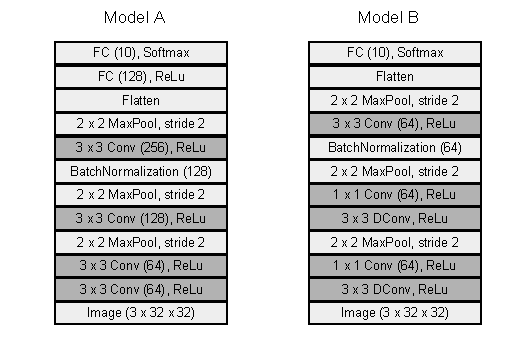
\includegraphics[width=0.5\textwidth]{../figures/models.pdf}
	\caption{CNN-based models for case study.}
	\label{fig:models}
\end{figure}

\subsection{Fixed-point models}
To evaluate the compute performance on fixed-point, we deploy model A and B with 8-bit fixed-point quantization. The compute performance on model A and B is presented in \tab{tab:performance_fixed_point}. A runtime execution of model A is illustrated in \fig{fig:sched_model_a_fixed}.

\begin{table}[!htp]\centering
	\caption{Compute performance with fixed-point on model A and B.}\label{tab:performance_fixed_point}
	\scriptsize
\begin{tabular}{lrrrrrrr}\toprule
	\multicolumn{2}{c}{\textbf{Tensor operation}} &\textbf{CPU} &\multicolumn{3}{c}{\textbf{TP (fixed-point)}} &\multirow{2}{*}{\textbf{Accel.}} \\\cmidrule{1-6}
	\textbf{Operation} &\textbf{MOP} &\textbf{t (ms)} &\textbf{t (ms)} &\textbf{MOP/s} &\textbf{GOP/W} & \\\midrule
	\multicolumn{2}{c}{\textbf{Model A}} & & & & & \\
	(1A) Conv &1.769 &700.22 &55.19 &32.06 &0.23 &\textbf{12.69} \\
	(2A) Conv &37.748 &12,666.91 &297.08 &127.06 &0.93 &\textbf{42.64} \\
	(3A) Conv &18.874 &6,081.01 &142.99 &131.99 &0.97 &\textbf{42.53} \\
	(4A) Conv &18.874 &5,543.77 &122.58 &153.97 &1.13 &\textbf{45.23} & \\\midrule
	\multicolumn{2}{c}{\textbf{Model B}} & & & & & \\
	(1B) DConv &0.027 &13.43 &0.63 &43.74 &0.25 &\textbf{21.25} \\
	(2B) Conv &0.196 &129.95 &11.57 &16.98 &0.12 &\textbf{11.23} \\
	(3B) DConv &0.147 &69.18 &3.33 &44.26 &0.25 &\textbf{20.77} \\
	(4B) Conv &1.048 &378.78 &9.96 &105.25 &0.77 &\textbf{38.02} \\
	(5B) Conv &2.359 &694.60 &16.46 &143.22 &1.05 &\textbf{42.20} \\
	\bottomrule
\end{tabular}
\end{table}

\begin{figure}[t!]
	\centering
	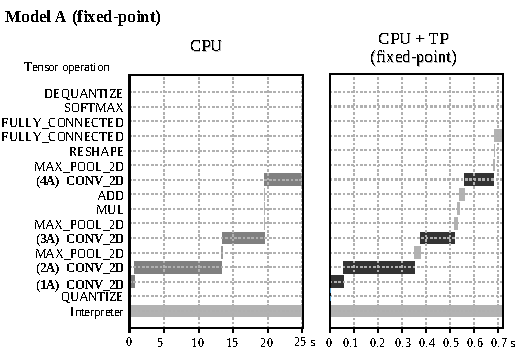
\includegraphics[width=0.5\textwidth]{../figures/sched_A_fixed_point.pdf}
	\caption{Compute performance with fixed-point on model A.}
	\label{fig:sched_model_a_fixed}
\end{figure}


\subsection{Floating-point models}
The compute performance with floating-point LogiCORE IP is presented in \tab{tab:performace_float_logicore}. The compute performance with hybrid custom floating-point approximation is presented in \tab{tab:performace_float_hybrid}. In these tables, we find the peak acceleration on the forth convolution operator of model A. The LogiCORE implementation accelerates 9.77X, and the proposed technique accelerates 44.87X, which is 4.59X faster.


\begin{table}[!htp]\centering
	\caption{Compute performance with floating-point LogiCORE on model A and B.}\label{tab:performace_float_logicore}
	\scriptsize
	\begin{tabular}{lrrrrrrr}\toprule
		\multicolumn{2}{c}{\textbf{Tensor operation}} &\textbf{CPU} &\multicolumn{3}{c}{\textbf{TP (floating-point LogiCORE)}} &\multirow{2}{*}{\textbf{Accel.}} \\\cmidrule{1-6}
		\textbf{Operation} &\textbf{MOP} &\textbf{t (ms)} &\textbf{t (ms)} &\textbf{MOP/s} &\textbf{GOP/W} & \\\midrule
		\multicolumn{2}{c}{\textbf{Model A}} & & & & & \\
		(1A) Conv &1.769 &670.95 &120.07 &14.73 &0.21 &\textbf{5.59} \\
		(2A) Conv &37.748 &12,722.13 &1,328.08 &28.42 &0.40 &\textbf{9.58} \\
		(3A) Conv &18.874 &6,094.85 &636.53 &29.65 &0.42 &\textbf{9.58} \\
		(4A) Conv &18.874 &5,564.79 &569.30 &33.15 &0.47 &\textbf{9.77} & \\\midrule
		\multicolumn{2}{c}{\textbf{Model B}} & & & & & \\
		(1B) DConv &0.027 &11.51 &1.557 &17.75 &0.23 &\textbf{7.39} \\
		(2B) Conv &0.196 &94.82 &20.487 &9.59 &0.13 &\textbf{4.62} \\
		(3B) DConv &0.147 &58.84 &8.355 &17.64 &0.23 &\textbf{7.04} \\
		(4B) Conv &1.048 &368.66 &40.271 &26.03 &0.37 &\textbf{9.15} \\
		(5B) Conv &2.359 &697.08 &72.981 &32.32 &0.46 &\textbf{9.55} \\
		\bottomrule
	\end{tabular}
\end{table}

\begin{table}[!htp]\centering
	\caption{Compute performance with hybrid custom floating-point approximation on model A and B.}\label{tab:performace_float_hybrid}
	\scriptsize
\begin{tabular}{lrrrrrrr}\toprule
	\multicolumn{2}{c}{\textbf{Tensor operation}} &\textbf{CPU} &\multicolumn{3}{c}{\textbf{TP (hybrid custom floating-point)}} &\multirow{2}{*}{\textbf{Accel.}} \\\cmidrule{1-6}
	\textbf{Operation} &\textbf{MOP} &\textbf{t (ms)} &\textbf{t (ms)} &\textbf{MOP/s} &\textbf{GOP/W} & \\\midrule
	\multicolumn{2}{c}{\textbf{Model A}} & & & & & \\
	(1A) Conv &1.769 &670.95 &68.50 &25.83 &0.39 &\textbf{9.8} \\
	(2A) Conv &37.748 &12,722.13 &307.83 &122.63 &1.85 &\textbf{41.33} \\
	(3A) Conv &18.874 &6,094.85 &147.97 &127.55 &1.93 &\textbf{41.19} \\
	(4A) Conv &18.874 &5,564.79 &124.03 &152.17 &2.30 &\textbf{44.87} & \\\midrule
	\multicolumn{2}{c}{\textbf{Model B}} & & & & & \\
	(1B) DConv &0.027 &11.51 &1.41 &19.63 &0.27 &\textbf{8.17} \\
	(2B) Conv &0.196 &94.82 &20.34 &9.43 &0.14 &\textbf{4.66} \\
	(3B) DConv &0.147 &58.84 &6.58 &22.41 &0.31 &\textbf{8.94} \\
	(4B) Conv &1.048 &368.66 &12.75 &82.23 &1.24 &\textbf{28.91} \\
	(5B) Conv &2.359 &697.08 &17.14 &137.68 &2.08 &\textbf{40.68} \\
	\bottomrule
\end{tabular}
\end{table}

For comparison, \fig{fig:sched_model_a_float} shows the runtime executions of model A with the proposed floating-point solutions. \fig{fig:sched_model_b_float} presents execution of model B, which incorporates separable convolutions with both Conv and DConv operations.

\begin{figure*}[t!]
	\centering
	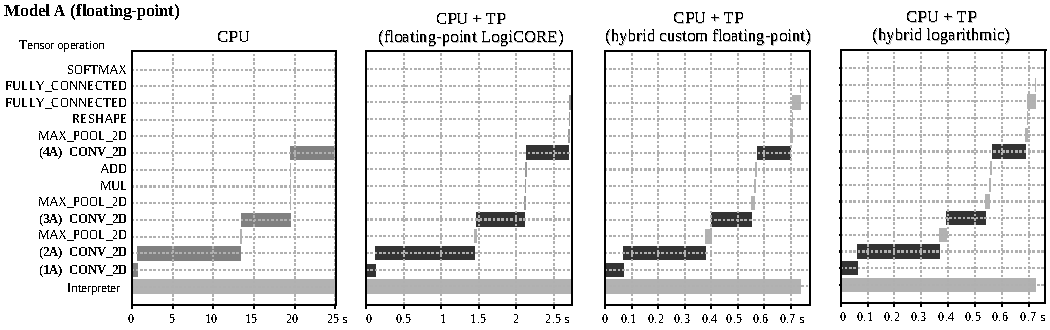
\includegraphics[width=\textwidth]{../figures/sched_A_float_all.pdf}
	\caption{Compute performance with the proposed floating-point solutions on model A.}
	\label{fig:sched_model_a_float}
\end{figure*}


\begin{figure}[t!]
	\centering
	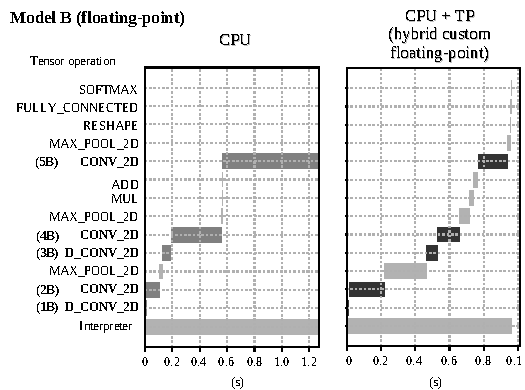
\includegraphics[width=0.5\textwidth]{../figures/sched_B_float.pdf}
	\caption{Compute performance on model B (floating-point).}
	\label{fig:sched_model_b_float}
\end{figure}

\subsection{Accuracy performance}

To evaluate the accuracy performance, we train A an B models for image classification with CIFAR-10 dataset. We deploy the models with a baseline accuracy of 76.6\% for model A, and 68.8\% for model B.

For accuracy evaluation, we implement the floating-point formats listed in \tab{tab:formats}. The base floating-point representation is quantized with bit-truncation and -rounding. The accuracy performance is presented in \fig{fig:accuracy}.

\begin{table}[!htp]\centering
	\caption{Implemented floating-point formats for accuracy evaluation.}\label{tab:formats}
	\scriptsize
	\begin{tabular}{lrrrrr}\toprule
		\multicolumn{5}{c}{\textbf{Floating-point formats}} \\\cmidrule{1-5}
		\textbf{Name} &\textbf{Size (bits)} &\textbf{Sign} &\textbf{Exponent} &\textbf{Mantissa} \\\midrule
		Logarithmic &6 &1 &5 &0 \\
		S1-E5-M1 &7 &1 &5 &1 \\
		S1-E5-M2 &8 &1 &5 &2 \\
		S1-E5-M3 &9 &1 &5 &3 \\
		S1-E5-M4 &10 &1 &5 &4 \\
		Float16 &16 &1 &5 &10 \\
		BFloat16 &16 &1 &8 &7 \\
		Tensor Float &19 &1 &8 &10 \\
		Float32 &32 &1 &8 &23 \\
		\bottomrule
	\end{tabular}
\end{table}

\begin{figure}[t!]
	\centering
	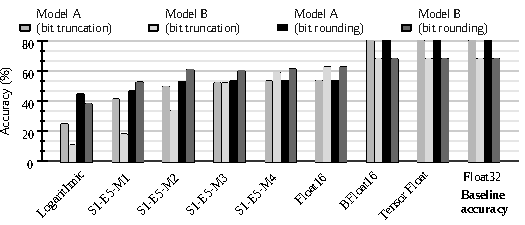
\includegraphics[width=0.5\textwidth]{../figures/all_models_accuracy.pdf}
	\caption{Accuracy performance using hybrid custom floating-point approximation with various formats.}
	\label{fig:accuracy}
\end{figure}

\subsection{Resource utilization and power dissipation}
The resource utilization and power dissipation of the TP is listed in \tab{tab:resource}. The implementations with hybrid custom floating-point and logarithmic approximation are the most power efficient.

The estimated power dissipation of the CPU is $1.4W$. The estimated power dissipation of the TP implementing Conv operator with hybrid custom floating-point is $66mW$. This implementation achieves a peak acceleration of $44.87\times$. This results in a peak power efficiency improvement of $951\times$.

The power dissipation of the Zynq device is presented in \fig{fig:power}.

\begin{table}[!htp]\centering
	\caption{Resource utilization and power dissipation of the proposed TP engines.}\label{tab:resource}
	\scriptsize
\begin{tabular}{lrrrrrr}\toprule
	\textbf{} &\multicolumn{4}{c}{\textbf{Post-implementation resource utilization}} &\multirow{2}{*}{\textbf{Power (W)}} \\\cmidrule{2-5}
	\textbf{TP engine} &\textbf{LUT} &\textbf{FF} &\textbf{DSP} &\textbf{BRAM 18K} & \\\midrule
	\multicolumn{6}{l}{\textbf{Fixed-point}} \\
	Conv &5,677 &4,238 &78 &70 &0.136 \\
	DConv &7,232 &5,565 &106 &70 &0.171 \\
	Conv + DConv &12,684 &8,015 &160 &70 &0.248 & \\\midrule
	\multicolumn{6}{l}{\textbf{Floating-point LogiCore}} \\
	Conv &4,670 &3,909 &59 &266 &0.070 \\
	DConv &6,263 &5,264 &82 &266 &0.075 \\
	Conv + DConv &10,871 &7,726 &123 &266 &0.119 \\\midrule
	\multicolumn{6}{l}{\textbf{Hybrid custom floating-point}} \\
	Conv &6,787 &4,349 &56 &74 &0.066 \\
	DConv &8,209 &5,592 &79 &74 &0.072 \\
	Conv + DConv &14,590 &8,494 &117 &74 &0.108 & \\\midrule
	\multicolumn{6}{l}{\textbf{Hybrid logarithmic}} \\
	Conv &6,662 &4,242 &54 &58 &0.060 \\
	DConv &8,110 &5,380 &77 &58 &0.066 \\
	Conv + DConv &14,370 &8,175 &113 &58 &0.105 \\
	\bottomrule
\end{tabular}
\end{table}

\begin{figure}[t!]
	\centering
	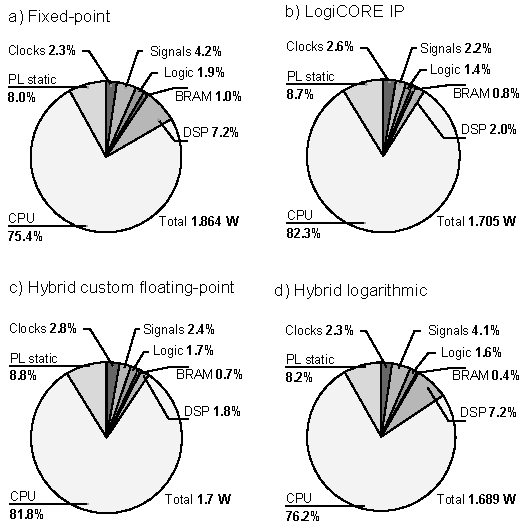
\includegraphics[width=0.5\textwidth]{../figures/power_breackdown.pdf}
	\caption{Estimated power dissipation of the Zynq-7020 SoC with different TP engines.}
	\label{fig:power}
\end{figure}

